\documentclass[a4paper, 12pt,oneside]{article}
\usepackage{graphicx} % Required for inserting images
\usepackage[top=2.5cm, bottom=2cm, left=2cm, right=2cm]{geometry}
\usepackage[T1]{fontenc}
\usepackage[utf8]{inputenc}
\usepackage[colorlinks,bookmarks=false,linkcolor=black,urlcolor=blue, citecolor=black]{hyperref}
\usepackage{units}
\usepackage{verbatim}
\usepackage{verbdef}% http://ctan.org/pkg/verbdef
\usepackage{amsmath}
\usepackage{amssymb}
\usepackage{wrapfig}
\usepackage{subcaption}
\usepackage{caption}
\usepackage{float}
\usepackage[export]{adjustbox}
\usepackage{upgreek}
\usepackage{hyperref}
%Pour changer la taille des titres de section et subsection. Ajoutez manuellement les autres styles si besoin.
\makeatletter
\renewcommand{\section}{\@startsection {section}{1}{\z@}%
             {-3.5ex \@plus -1ex \@minus -.2ex}%
             {2.3ex \@plus.2ex}%
             {\normalfont\normalsize\bfseries}}
\makeatother

\makeatletter
\renewcommand{\subsection}{\@startsection {subsection}{1}{\z@}%
             {-3.5ex \@plus -1ex \@minus -.2ex}%
             {2.3ex \@plus.2ex}%
             {\normalfont\normalsize\bfseries}}
\makeatother

\graphicspath{{Graphes/}}


\title{Travaux Pratiques n°H5: Rayons X}
\author{Groupe n°22: Armand Le Douarec Maxime Chatelin}
\date{3 Octobre 2024}

\begin{document}
\title{\normalsize{Lab Work Report - Group N$^\circ$\\ XX - Experiment}}
\date{\normalsize{\today}}
\author{\normalsize{Name} 1\and \normalsize{Name 2}}

\begin{center}
\large\textbf{\sffamily Expérience N$^\circ$H5. Rayons X}\\%
\large\sffamily Groupe N$^\circ$22: Armand Le Douarec, Maxime Chatelin\\%
\large\sffamily\today\quad   Assistant -  Sylvain Mortgat \\%
\end{center}

\section{Introduction}

Les rayons X, découverts par Wilhelm Röntgen en 1895, sont rapidement devenus un outil fondamental dans de nombreux domaines scientifiques et technologiques. Leur capacité unique à pénétrer la matière, combinée à des phénomènes comme l’absorption et la diffraction, les rend indispensables en médecine pour l’imagerie médicale [\ref{ref1}], en biophysique pour l’étude des structures moléculaires [\ref{ref2}] et en microélectronique pour l’analyse des matériaux [\ref{ref3}]. Au-delà de ces applications, les rayons X ont aussi révolutionné la science des matériaux en permettant la caractérisation précise des structures cristallines, ouvrant ainsi la voie à des avancées majeures dans le développement de nouveaux matériaux et technologies [\ref{ref4}]. Ce travail pratique s’inscrit dans cette dynamique, en étudiant les mécanismes de production et d’interaction des rayons X avec différents types de matière.\\
Les expériences se concentrent sur la réponse du tube compteur Geiger-Müller en fonction de l'intensité de ces rayons et la tension d'accélération appliquée lors des expériences, la diffraction des rayons X au sein de cristaux, notamment un cristal de NaCl, et enfin l’absorption de ces rayons dans des épaisseurs et matériaux variés.
\vspace{-0.23cm}

\section{Théorie}
\vspace{-0.17cm}
\paragraph{Définition}

Les rayons X sont des rayonnements électromagnétiques dont la fréquence varie entre $10^{17}\,$Hz et $10^{20}$ \,Hz [\ref{ref5}]. Ils sont émis lorsque des perturbations d'électrons se produisent dans les couches électroniques internes de l'atome. L'effet est obtenu en bombardant un matériau avec des électrons à très grande vitesse. Dès lors, deux types de rayonnements X se distinguent par leurs effets sur l'atome atteint.

Dans le premier cas de figure, les électrons passent près du noyau sans provoquer d’ionisation. L’énergie perdue lors de leur freinage, causée par la force électromagnétique, est convertie sous forme de rayonnement des photons émis. L’énergie totale $h\nu$ de ces photons est ainsi toujours inférieure ou égale à l’énergie cinétique $eV$ de l’électron. L'équation ainsi établie donne [\ref{ref5}]:

\begin{equation}
    h\nu=h\frac{c}{\lambda} \leq eU
    \implies \lambda_{min} = \frac{c}{v_{max}} = \frac{ch}{eU}
    \label{eq1}
\end{equation}

avec $h$ = 6.626 · $10^{-34}$ J·s la constante de Planck [\ref{ref6}], $\nu$ la fréquence des oscillations de l’onde élecromagnétique émise, $\lambda$ sa longueur d’onde, $c$ = 2.998 · $10^8$ m/s la vitesse de la lumière [\ref{ref7}],
$e$ = 1.602 · $10^{-19}$ C, la charge élémentaire de l’électron [\ref{ref8}] et $U$ la tension d’accélération.\\

L'autre cas se produit dès lors que les électrons pénétrant à l'intérieur de l'atome l'ionisent en arrachant un électron d'une couche inférieure. Un électron d'une couche supérieure prend alors la place de l'électron arraché pour maintenir un état stable. Le mouvement de l'électron induit l'émission d'un rayonnement électromagnétique dont la fréquence est directement proportionnelle à la différence entre les énergies de l'électron avant et après son passage d'une couche à l'autre [\ref{ref5}].\\

\paragraph{Diffraction}
Une fois émis ces rayonnements se caractérisent par leur propriétés telles que leur diffraction dans les cristaux et leur absorption. En effet, un cristal fonctionne comme une série de plans parallèles qui diffractent les rayons X. Des interférences constructives ou destructives sont ainsi crées, générant alors un motif de diffraction. Les constructives ont lieu lorsque la différence de chemin parcouru par deux ondes réfléchies par deux plans consécutifs est un multiple de $\lambda$ la longueur d'onde. La loi de Bragg s'établit alors à travers la formule [\ref{ref5}]:
\vspace{-0.2cm}
\begin{equation}
    2d\sin{\theta}=n\lambda
\label{eq2}
\end{equation}
\vspace{-0.05cm}
avec $2d$ = 5.640 · $10^{-8}$\,m la distance entre deux plans consécutifs du cristal de NaCl [\ref{ref9}], $\theta$ l'angle d'incidence du rayon X et $n$ un entier.\\

\paragraph{Absorption}
Quant à l'absorption des rayons X, le passage à travers de la matière génère une diminution de l'intensité des rayons corrélée à l'augmentation de l'épaisseur $d$ d'un matériau. Cette même diminution est aussi affectée par matériau utilisé, identifié par son numéro atomique [\ref{ref5}]. Étant donné la relation linéaire supposée entre la réponse du rayonnement $R$ et l'intensité du rayonnement $I$ donnée par $R= pI$. Les relations liées à ce phénomène [\ref{ref5}] sont les suivantes:
\vspace{-0.15cm}
\begin{equation}
    I=I_0e^{-md} \Rightarrow
    R=R_0e^{-md}
\label{eq3}
\end{equation}
\vspace{-0.05cm}
avec $I_0$ l'intensité à vide, $m$ le coefficient d'absorption du matériau et $R_0$ la réponse à vide.\\
\paragraph{Effet Compton}Enfin, l'effet Compton explique la collision entre un photon de rayonnement X et un électron libre. L'électron récupère alors l'énergie du photon sous forme d'énergie cinétique [\ref{ref5}].
\vspace{-0.2cm}
\section{Démarche expérimentale}
\vspace{-0.2cm}
\paragraph{Réponse du Tube compteur Geiger-Müller}
Dans ces travaux pratiques, l'outil principal est un tube compteur Geiger-Müller [\ref{ref5}] afin de détecter et mesurer les radiations ionisantes. Ce dispositif cylindrique est principalement composé de molybdène, matériau bombardé par les rayons X, d'un fil et d'un gaz sous faible pression. Son fonctionnement repose sur l'ionisation du fil lorsque des particules ionisantes le traversent, provoquant ainsi une décharge électrique. Cette décharge est enregistrée sous forme d'impulsions, permettant enfin de compter les particules traversant le tube.

La première expérience, essentielle pour les expériences qui suivent, met en évidence la réponse $R$ du tube compteur en fonction de l'intensité de courant variant de $I=(0.000\,\pm\,0.005)\,$mA à $I=(1.000\,\pm\,0.005)\,$mA, pour les tensions fixées $U=([20.00,25.00,30.00,35.00]\pm0.05)$\,kV. \\
La seconde expérience permet une calibration plus détaillée du tube compteur et de trouver ses limites. La tension est fixée à $U=(30.0\pm0.05)$\,kV tandis que le courant varie entre $I=(0.000\,\pm\,0.005)\,$mA et $I=(0.100\,\pm\,0.005)\,$mA. Dans ces expériences, à chaque intensité, les valeurs minimale et maximale de la réponse du tube GM sont relevées sur un intervalle $t=(10\,\pm\,1)$\,s. La réponse mesurée est la moyenne de ces deux valeurs.
\vspace{-0.2cm}

\paragraph{Expérience de Bragg}
L'expérience met en lumière la réponse du tube compteur avec $\theta$ variant de (2.50$\,\pm\,0.05)$° à (25.00$\,\pm\,0.05)$° avec un pas de 0,1° entre chaque mesure. De plus, les mesures sont faites pour $U=([20.00,25.00,30.00,35.00]\pm0.05)$\,kV et $I=(0.700\pm 0.005)$\,mA.
Découle de cette expérience le diffractogramme du cristal, permettant ainsi d'en déduire la longueur d'onde des raies d'émission $K_{\alpha}$ et $K_{\beta}$ du molybdène, le matériau dans l'anticathode. En outre, à l'aide de l'équation (\ref{eq1}), une approximation de la constante de Planck $h$ est permise.
\clearpage
\paragraph{Absorption en fonction de l'épaisseur et du nombre atomique}

Pour mesurer R en fonction de différentes épaisseurs, il est judicieux d'utiliser une coque cylindrique comportant sept fentes, une vide et six complétées par des plaques d’aluminium d’épaisseurs variables, allant de $d=(0.50\,\pm\, 0.15)$\,mm à $d=(3.00\,\pm\, 0.15)$\,mm. Par pivotation de la coque, la réponse moyenne de chaque échantillon d'aluminium est enregistrée à l'aide du tube GM. Les paramètres sont fixés à $U=(30.0\,\pm\,0.05)$\,kV et $I=(0.020\,\pm\,0.005)$\,mA tandis que $\theta$, l'angle de rotation de la coque varie entre (-2.50$\,\pm\,0.05)$° et (65.00$\,\pm\,0.05)$° avec un pas de 0.1°. 

Ensuite, la mesure de R en fonction du matériau, est effectuée via le même dispositif. Cinq différents matériaux sont employés: le plastique ($Z = 6$), Al ($Z = 13$), Fe ($Z = 26$), Cu ($Z = 29$), Zr ($Z = 40$),($Z = 47$), tous d'épaisseur $d=(0.50\,\pm\, 0.05)$\,mm. À partir de ces tests, les coefficients d'absorption des différents matériaux utilisés sont estimés. De nouveau, à chaque épaisseur ou chaque matériau, les valeurs minimale et maximale de la réponse du tube GM sont relevées sur le graphe. La réponse mesurée est la moyenne de ces deux valeurs.
\vspace{-0.5cm}

\paragraph{Paramètre de maille d'un cristal inconnu}
Dans cette expérience est répétée l'expérience de Bragg déjà effectuée, Il s'agit ici d'un cristal de LiF. Le paramètre de maille $d$ du LiF est inconnu et est déduit du diffractogramme du LiF établi, toujours avec du molybdène dans l'anticathode. Les longueurs d'onde des raies d'émission $K_{\alpha}$ et $K_{\beta}$ connues, combinées à l'équation (\ref{eq2}) fournissent une estimation de $d$. Les paramètres de l'expérience sont $U=(30.0\pm0.05)\,$kV et $I=(0.700\,\pm\,0.005)$\,mA avec $\theta$ variant de (2.50$\,\pm\,0.05)$° à (25.00$\,\pm\,0.05)$° par pas de 0.1°.
\vspace{-0.5cm}

\paragraph{Effet Compton}
Pour mettre en évidence cet effet, il est d'usage d'utiliser une feuille de cuivre, comparable à un filtre, ne laissant passer que les photons ayant une vitesse suffisamment grande (dépassant une vitesse limite).
 La feuille est d'abord placée devant le diffuseur, puis devant le tube compteur. Une plaque d'aluminium a pour fonction de laisser les photons s'y heurter et donc de provoquer l'effet Compton. Dans le premier cas, une partie des photons — les plus rapides — passe le filtre, heurte la plaque et sont ralentis mais sont tout de même captés par le tube compteur. Dans le second cas, tous les photons heurtent la plaque, sont ralentis puis arrivent au tube GM et, de par l'effet Compton, ils sont alors plus lents que dans le premier cas lorsqu'ils parviennent au filtre. Donc, moins de photons passent la feuille de Cu. Le capteur accumule les radiations X pendant une durée de $t = (600.0 \pm 0.5)$\,s, avec un courant de $I = (1.000\,\pm\,0.005)$\,mA et une tension de $U = (30.0\,\pm\,0.05)$\,kV.
\vspace{-0.5cm}
\section{Résultats}
\vspace{-0.8cm}
\begin{figure}[H]
\begin{subfigure}{0.45\textwidth}  % Réduire la taille pour s'assurer qu'elles tiennent côte à côte
    \centering  % Centrer cette sous-figure
    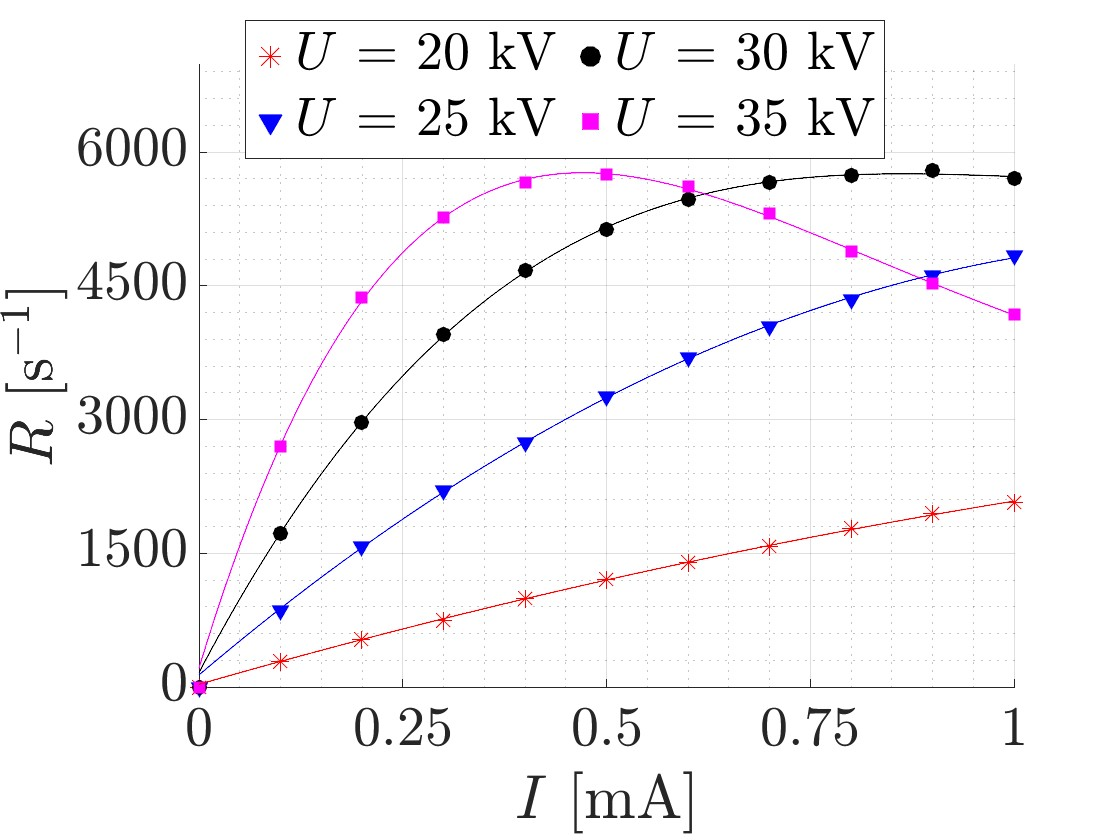
\includegraphics
    [scale=0.21]{Graphes/new_new_1.jpg}
    \vspace{-1cm}
    \captionsetup{justification = raggedright,font = large}
    \caption{\phantom{-------------}}
    \label{fig1a}
\end{subfigure}
\hspace{0.05\textwidth}
\begin{subfigure}{0.45\textwidth}  % Réduire également ici
    \centering  % Centrer cette sous-figure
    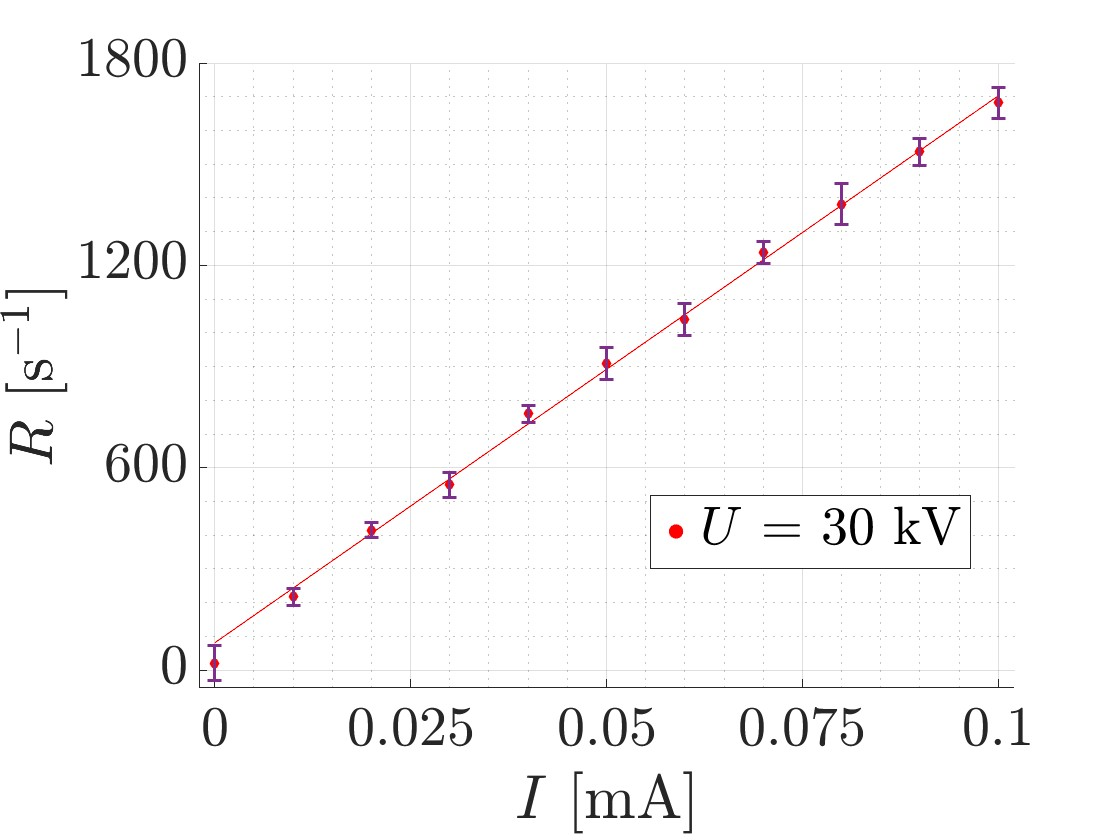
\includegraphics[width=1.1\linewidth, height = 5.8cm]{Graphes/new_2.jpg}
    \vspace{-1cm}
    \captionsetup{justification = raggedright,font = large}
    \caption{\phantom{-------------}}
    \label{fig1b}
\end{subfigure}
\vspace{-0.3cm}
\captionsetup{justification=centering}
\caption{(a) Réponse $R$ en fonction du courant $I$ pour différentes tensions d'accélération $U=([20.00,25.00,30.00,35.00]\pm0.05)$\,kV. (b) Réponse $R$ en fonction du courant $I$ pour une calibration plus détaillée avec une faible intensité $I$ variant de ($0.000\,\pm\, 0.005)\,$mA à ($0.100\,\pm\, 0.005)\,$mA et un fit linéaire de pente $p$=(1.6$\,\pm\,$0.5$)\,$(mA\,s)$^{-1}$.}
\label{fig1}
\end{figure}
\clearpage
\paragraph{Réponse du tube compteur Geiger-Müller}
Sur la Fig.(\ref{fig1a}), pour $I$ allant de (0.000$\,\pm\,$0.005)\\mA à (1.000$\,\pm\,$0.005)\,mA, plusieurs fits sont effectués : fit de degré 4 pour $U=(35\pm0.05)$\,kV,  degré 3 pour $U=(30\pm0.05)$\,kV, degré 2 pour $U=(25\pm0.05)$\,kV, degré 2 pour $U=(20\pm0.05)$\,kV. Dans la Fig.(\ref{fig1b}), la réponse est évaluée avec une intensité plus faible, $I$ variant entre  (0.000$\,\pm\,$0.005)\,mA (0.10$\,\pm\,$0.005)\,mA, pour effectuer une calibration détailllée. Sur la Fig.(\ref{fig1b}) un fit linéaire est apppliqué entre la réponse et l’intensité, il correspond à la relation $R=pI$ avec $p=(1.6\,\pm\,0.5)$ · 10$^4$\,(mA·s)$^{-1}$.
\vspace{-0.4cm}
\paragraph{Expérience de Bragg}
\setlength{\intextsep}{5pt}

\begin{wrapfigure}{h}{0.5\textwidth}
\vspace{-1cm}
    \centering
    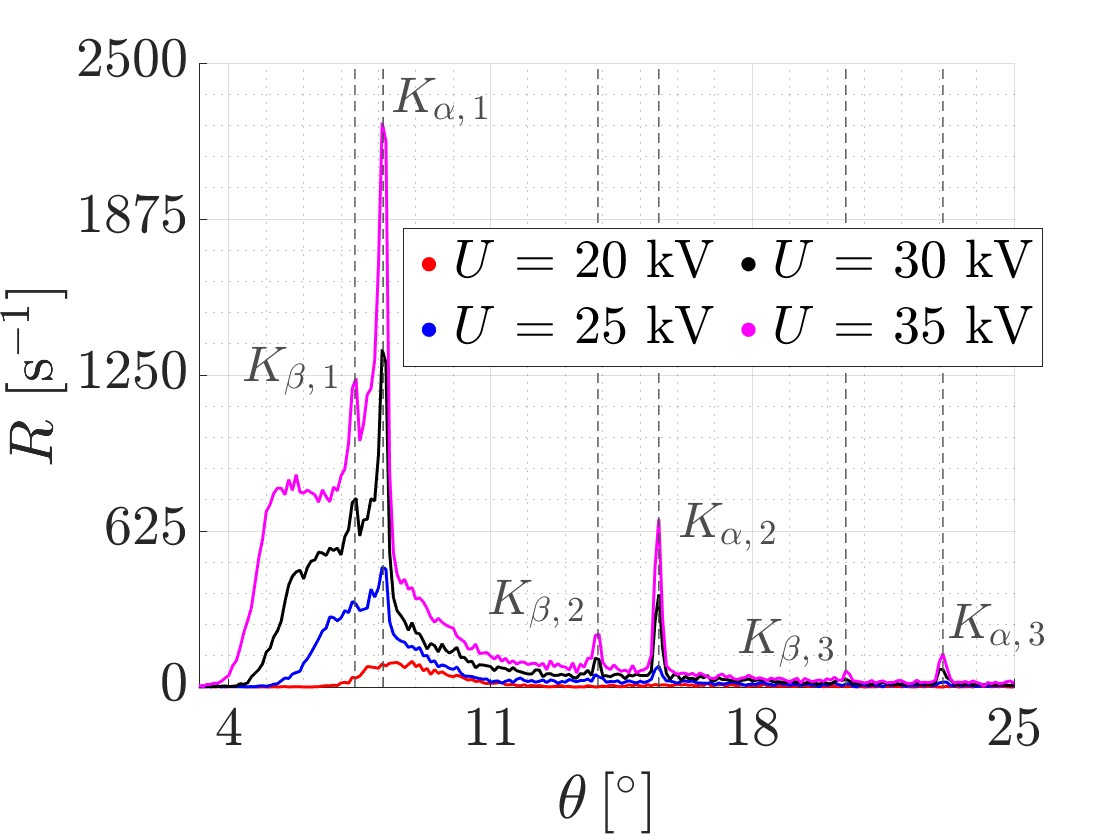
\includegraphics[width=1\linewidth]{Graphes/Bragg.jpg}
    \captionsetup{justification=centering}
    \caption{Diffractogramme du NaCl pour différentes tensions et mise en évidence des raies d'émission $K_{\alpha,n}$ et $K_{\beta,n}$, avec $n=1,2,3$.}
    \label{fig2}
\end{wrapfigure}

La Fig.(\ref{fig2}) présente les raies d'émission $K_{\alpha,n}$ et $K_{\beta,n}$, avec $n=1,2,3$. 
En utilisant l'équation (\ref{eq2}) et la valeur de référence du paramètre de maille $d$ du NaCl, les longueurs d'onde $\lambda$ correspondantes sont calculées et inscrites dans le Tab.(\ref{tab1}).

De plus, la plus petite valeur d'angle à partir de laquelle une réponse du tube compteur a lieu, appelé $\theta_{min}$, est relevée. Celle-ci et l'équation (\ref{eq1}) permettent de trouver la constante de Planck. Elle est en moyenne estimée à $h=(6.5\pm0.14)$·10$^{-34}$\,J·s. Les résultats sont inscrits dans le Tab.(\ref{tab2}). Les incertitudes de ces angles sont déterminées à la vue du graphe, lorsque $R(\theta)>5\,$ s$^{-1}$.

\begin{table}[h]
\centering
\begin{tabular}{|c||c|c|c|c|c|c|}
\hline
Raies & $K_{\beta ,\,1}$ & $K_{\alpha ,\,1}$ & $K_{\beta ,\,2}$ & $K_{\alpha ,\,2}$ & $K_{\beta ,\,3}$ & $K_{\alpha ,\,3}$ \\
\hline
$\theta$ [°] & $7.35\,\pm 0.05$ & $8.12\,\pm 0.05$ & $13.87\,\pm 0.05$ & $15.50\,\pm 0.05$ & $20.50\,\pm 0.05$ & $23.10\,\pm 0.05$ \\
\hline
$\lambda$ [pm] & $72.2\,\pm 0.5$ & $79.7\,\pm 0.5$ & $67.5\,\pm 0.2$ & $75.4\,\pm 0.2$ & $65.84\,\pm 0.15$& $73.75\,\pm 0.15$ \\
\hline
\end{tabular}
\captionsetup{justification=centering}
\caption{Angles de diffraction $\theta$ et longueurs d'onde $\lambda$ associées des raies d'émission $K_\alpha$ et $K_\beta$\\
Valeur moyenne de la longueur d'onde $\lambda_{moy} = (72.4\,\pm\,1.7)\,$pm}
\label{tab1}
\end{table}

\begin{table}[h]
\begin{tabular}{|c|c|c|c|}
\hline
$U$ [kV] & $\theta_{min}$ [°]  & $h$ [J$\,$s$\times 10^{-34}$] & $\epsilon_{h,\text{rel.}}$ [\%] \\
\hline
\hline
$20.00\,\pm 0.05$& $6.5\,\pm 0.4$ & $6.8\,\pm 0.4$ & 3 \\
\hline
$25.00\,\pm 0.05$& $4.8\,\pm 0.4$ & $6.3\,\pm 0.5$ & 5 \\
\hline
$30.00\,\pm 0.05$& $4.2\,\pm 0.2$ & $6.6\,\pm 0.3$ & 0.4 \\
\hline
$35.00\,\pm 0.05$& $3.4\,\pm 0.3$ & $6.3\,\pm 0.5$ & 5 \\
\hline
\end{tabular}
\captionsetup{justification=raggedleft}
\vspace{-3cm}
\caption{Angle minimum $\theta_{min}$ enregis-\\trant une réponse et constante de Planck \\$h$ associée avec erreur relative $\epsilon_{h,\text{rel.}}$ par\\rapport à la valeur de référence $h_{ref}$ [\ref{ref6}]\\ différentes tensions d'accélération $U$}
\label{tab2}
\end{table}
\vspace{-0.4cm}
\paragraph{Absorption en fonction de l'épaisseur}
\begin{wrapfigure}{r}{0.5\textwidth}
\vspace{-2cm}% 'r' pour aligner à droite, '0.45\textwidth' pour la largeur du wrap
    \centering  % Centrer l'image
    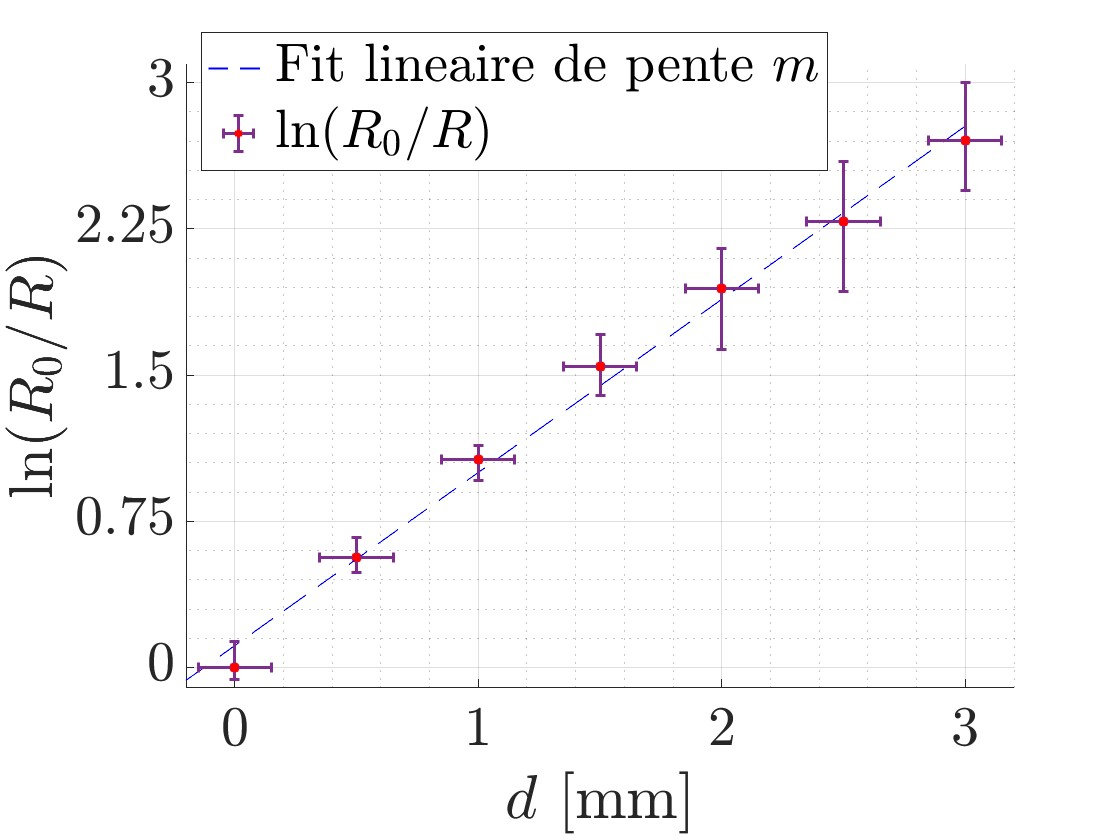
\includegraphics[scale=0.2]{Graphes/Fit_absorption_epaisseur.jpg}
    \captionsetup{justification=centering}
    \caption{Graphe du logarithme de $R_0/R$ en fonction de l'épaisseur $d$ de la plaque et fit linéaire de pente $m=(0.89\,\pm\,0.08)$\,mm$^{-1}$.}
    \label{fig3}
    \vspace{-1.11cm}
\end{wrapfigure}
En opérant à courant faible, la relation $R=pI$\\ trouvée dans la première expérience fonctionne.

 La Fig.(\ref{fig3}) permet d'étudier $\ln(R_0/R)$ en fonction de l'épaisseur $d$. L'équation (\ref{eq3}) expose l'égalité entre la pente du fit linéaire effectué dans cette figure et le coefficient d'absorption $m$ de l'aluminium. Le résultat de ce coefficient est donc $m=(0.89\,\pm\,0.08)$\,mm$^{-1}$.
\vspace{-0.25cm}
\paragraph{Absorption en fonction du numéro atomique}
Le Tab.(\ref{tab3}) affiche les réponses moyennes $R$ du tube compteur. A partir de l'équation (\ref{eq3}), il est possible de trouver le coefficient $m$ et de le comparer à la valeur de référence. A partir du Fe ($Z = 26$), l'intensité, étant trop faible pour mesurer une réponse valide a été augmentée avec $I=(0.50\pm0.005)$\,mA et il a été supposé que le courant se situe dans la plage linéaire. Les graphiques présentant la réponse en fonction du numéro atomique et de l'épaisseur sont laissés en annexe.

\begin{table}[h]
\begin{tabular}{|c||c|c|c|c|c|c|c|}
\hline
$Z$ & 6 & 13 & 26 & 29 & 40 & 47 \\
\hline
$R$ [s$^{-1}$] & $1810\,\pm 30$ & $1130\,\pm 20$ & $12\,\pm 8$ & $2\,\pm 1$& $28\,\pm 5$ & $7\,\pm 4$ \\
\hline
$m$ [mm$^{-1}$] & $0.18\,\pm 0.05$ & $1.12\,\pm 0.05$ & $12.1\,\pm 1.5$ & $16\,\pm 2$ & $10.4\,\pm 0.4$& $13.2\,\pm 1.5$ \\
\hline
$m_{\text{ref}}$ [mm$^{-1}$]& $0.52\pm 0.05$ & $0.6\,\pm 0.3$& $5\,\pm 2$& $7\,\pm 3$& $12\,\pm 4$& $28\,\pm 10$\\
\hline
$\epsilon_{m\text{, rel}}$ [\%]&65&87&140&129&13&54\\
\hline
\end{tabular}
\captionsetup{justification=centering}
\caption{Coefficients d'absorptions $m$ en fonction du numéro atomique $Z$ et erreur relative $\epsilon_{m\text{, rel}}$ des résultats par rapport à la valeur de référence $m_{ref}$}
\label{tab3}
\end{table}
\vspace{-0.4cm}
\paragraph{Paramètre de maille d'un cristal inconnu}


\begin{wrapfigure}{r}{0.5\textwidth}
    \centering
    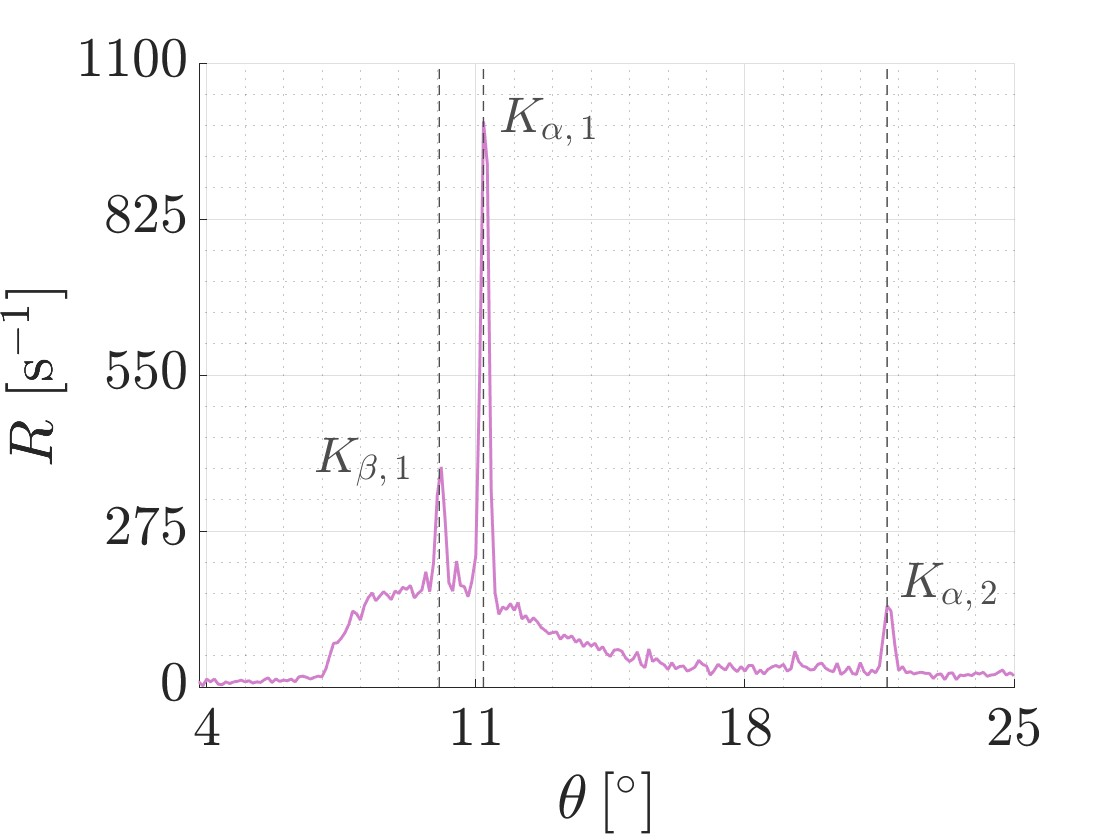
\includegraphics[width=1\linewidth]{Graphes/Unknown_cristal.jpg}
    \captionsetup{justification=centering}
    \caption{Diffractogramme du cristal de LiF pour la tension d'accélération $U=(30.0\pm0.05)\,$kV et une intensité $I=(0.700\,\pm\,0.005)$\,mA. Mise en évidence des raies d'émission $K_{\alpha,n}$ et $K_{\beta,n}$, avec $n=1,2,3$.}
    \label{fig4}
\end{wrapfigure}

La Fig.(\ref{fig4}) montre le diffractogramme du LiF. Grâce aux résultats de la précédente expérience de Bragg et l'équation (\ref{eq2}), le paramètre de maille $d$ du LiF peut être déterminé. Pour effectuer ce calcul, les raies d'émission sont trouvées sur le graphe aux pics du diffractogramme, $K_{\alpha,1}$, ici, $\theta_{\alpha,1}=(11.20\pm0.05)$\,°. D'après le Tab.(\ref{tab1}), $\lambda_{\alpha,1}=(79.7\pm0.5)$\,pm. Ainsi, le résultat est $d=(2.1\pm 0.5)$\,Å. Le paramètre de maille du LiF est de (4.2$\,\pm\,1.0)\,$Å. L'erreur relative avec la valeur de référence de 4,03\,Å est de 4\%.
\vspace{-0.4cm}
\paragraph{Effet Compton}

Avec l'utilisation d’un filtre en cuivre sur le collimateur, la réponse moyenne est $R=(1.39\,\pm\,0.06)$\,s$^{-1}$, alors qu'en plaçant le filtre en cuivre sur le logement du capteur, le résultat final est $R=(1.20\,\pm\,0.06)$\,s$^{-1}$.
\vspace{-0.3cm}
\section{Discussion}
\vspace{-0.3cm}

\paragraph{Tube compteur GM}
Les premières expériences, rapportées sur les Fig.(\ref{fig1a}) et Fig.(\ref{fig1a}), mettent en évidence les points de saturation du tube compteur GM. La Fig.(\ref{fig1a}) permet de constater que l'augmentation de la tension d’accélération $U$ implique l'augmentation la réponse $R$ du tube compteur. Malgré l'augmentation de la réponse pour chaque augmentation de la tension d'accélération, il est essentiel de souligner que la réponse $R$ atteint un maximum, $R_{sat}$ qui ne peut être dépassé lorsque $U=([30.00,35.00]\pm0.05)$\,kV. $R_{sat}$ vaut ($5810\,\pm\,50)$\,s$^{-1}$, par lecture du graphe Fig.(\ref{fig1a}), pour ce tube GM. Tant que la réponse saturante $R_{sat}$ n’est pas atteinte, il est clair que l’augmentation du courant $I$ implique l’augmentation de la réponse $R$. $R$ dépendrait donc de $U$ et $I$. Dans la continuité de ces suppositions, la réponse saturante pourrait être atteinte pour $U=(25.00\pm0.05)$\,kV avec une intensité plus forte. Une des raisons de cette saturation est liée aux limites du tube compteur. En effet, le tube Geiger-Müller possède un temps mort entre chaque détection de décharge électrique. Lorsque trop d’impulsions électriques sont causées par les rayons X pendant un court instant, le tube ne parvient pas à toutes les repérer et à correctement les quantifier. Ce temps mort induit une paralysie de comptage qui peut affecter la qualité des résultats obtenus. Dans le cas de ce tube compteur, il est complexe de dévier cette difficulté liée à la limite même de l'appareil. Sur les mêmes figures Fig.(\ref{fig1a}) et Fig.(\ref{fig1b}), les fits linéaires donnent une approximation intéressante de la réponse en fonction de l'intensité. En effet, d'après la Fig.(\ref{fig1b}), la tension d'accélération joue un rôle clé dans le comportement de la réponse du tube. Lorsqu'elle croît, la réponse du tube suit de moins en moins la relation linéaire $R = pI$. Le témoigne les degrés des fits employés à chaque tension d'accélération qui sont de plus en plus grands. Pour exploiter cette relation, il est donc nécessaire de se limiter à une faible intensité, en particulier pour correctement analyser l'absorption de rayons X selon l'épaisseur et le matériau Fig.(\ref{fig3}) et Tab.(\ref{tab3}).
\vspace{-0.35cm}
\paragraph{Mesure du diffractogramme du rayon X à différentes tensions}
La Fig.(\ref{fig2}) du diffractogramme du NaCl met en évidence les raies $K_\alpha$ et $K_\beta$ de l’anticathode en molybdène. Il est essentiel de noter que les longueurs d’onde associées aux raies d’émission ne dépendent aucunement de la tension d’accélération. D’autre part, cette expérience permet de trouver une approximation de la constante de Planck $h$. À partir des angles $\theta_{min}$, la réponse du tube est non nulle, pour une tension d'accélération donnée. Malgré les difficultés à relever ces angles avec une faible incertitude, il est important de noter que l'angle minimal diminue lorsque la tension d'accélération augmente. L'équation (\ref{eq1}) donne à partir de ces angles une valeur pour la constante de Planck $h$. Dans le Tab.(\ref{tab2}), l’erreur relative moyenne du résultat est finalement  de 1.8\%, ce résultat affirme que les valeurs expérimentales et les calculs sont conformes avec la théorie. L'erreur est probablement due à une imprécision dans la mesure des angles $\theta$ sur la Fig.(\ref{fig2}). Pour améliorer le résultat, il serait utile de répéter l'expérience avec différents cristaux, et d'effectuer une moyenne des valeurs trouvées.
\vspace{-0.35cm}
\paragraph{Absorption en fonction de l’épaisseur}
Les résultats sur la Fig.(\ref{fig3}) indiquent que la décroissance de la réponse est bien exponentielle en fonction de l’épaisseur comme intitulé dans l’équation (\ref{eq2}).
\vspace{-0.35cm}
\paragraph{Absorption en fonction du nombre atomique}
Le Tab.(\ref{tab3}) montre que le coefficient d’absorption $m$ augmente avec le nombre atomique sauf pour Zr($Z=40$),($Z=47$). La croissance de l'erreur relative peut être expliquée par les imprécisions des mesures qui fluctuent ou encore puisque ces matériaux absorbent la plupart des rayons X. Le bruit ou les moindres changements de réponse influent beaucoup sur la valeur de la réponse retenue et l'incertitude de cette donnée; par conséquent, sur la fiabilité des données. Ainsi, à cause de sa faible précision, la réponse du tube compteur a une utilité moindre pour les matériaux très absorbants comme le montre l'erreur relative élevée pour les métaux.
\vspace{-0.35cm}
\paragraph{Paramètre de maille d’un cristal inconnu}
En comparant le paramètre de maille trouvé, $2d=(4.2\pm1.0)$\,Å avec la valeur de référence du paramètre de maille du LiF \ref{ref10} de $2d=4.03$\,Å, L’erreur relative de 4\% souligne la précision du diffractogramme. Le tube GM s'avère utile pour la vérification ou l'identification de cristaux.
\vspace{-0.35cm}
\paragraph{Effet Compton}
Les rayons X étaient davantage absorbés lorsque la feuille de cuivre était placée après le diffuseur plutôt qu'avant. Cela correspond aux attentes liées à l'effet Compton: les rayons diffusés possèdent après impact une longueur d'onde plus grande, donc une énergie plus faible, ce qui les rend moins susceptibles de passer l’absorbant et d’être mesurés par le tube compteur.
\vspace{-0.3cm}
\section{Conclusion}
\vspace{-0.2cm}
Ainsi, ces travaux pratiques ont permis d'explorer en profondeur la nature des rayons X, leurs propriétés et leurs effets. L'utilisation essentielle du tube compteur Geiger-Müller a permis de mesurer et de quantifier ces rayonnements. La diffraction des rayons X sur des cristaux tels que le NaCl et le LiF a conduit à la détermination des longueurs d'onde des raies d'émission du molybdène, de la constante de Planck $h$, ainsi que du paramètre de maille $d$ du fluorure de lithium. L'absorption de ces rayons par différents matériaux, pour des épaisseurs variées, a également été étudiée, permettant de déterminer le coefficient d'absorption de l'aluminium. Enfin, l'étude de l'impact de ces rayons sur un matériau a mis en évidence l'effet Compton, manifestant un ralentissement des rayons X. Les principales caractéristiques des rayons X ont été présentées, offrant une meilleure compréhension de leur utilité dans divers domaines, notamment en cristallographie.

 
\section{Références}
\renewcommand{\labelenumi}{[\theenumi]}
\begin{enumerate}
    \item \label{ref1} OFSP, Application des rayonnements en radiologie\\
    \href{https://www.bag.admin.ch/bag/fr/home/gesund-leben/umwelt-und-gesundheit/strahlung-radioaktivitaet-schall/strahlenanwendungen-in-der-medizin/strahlenanwendungen-in-der-radiologie.html}{https://www.bag.admin.ch/bag/fr/home/gesund-leben/umwelt-und-gesundheit/strahlung-radioaktivitaet-schall/strahlenanwendungen-in-der-medizin/strahlenanwendungen-in-der-radiologie.html}
    \item \label{ref2} Wikipedia, Biophysique\\
    \href{https://fr.wikipedia.org/wiki/Biophysique}{https://fr.wikipedia.org/wiki/Biophysique}
    \item \label{ref3} IAEA, La Spectrométrie X\\
    \href{https://www.iaea.org/fr/science-nucleaire/la-spectrometrie-x}{https://www.iaea.org/fr/science-nucleaire/la-spectrometrie-x}
    \item \label{ref4} CNRS, Explorer la matière grâce à la micro-diffraction de rayons X\\
    \href{https://www.iledefrance-gif.cnrs.fr/fr/cnrsinfo/explorer-la-matiere-grace-la-micro-diffraction-de-rayons-x}{https://www.iledefrance-gif.cnrs.fr/fr/cnrsinfo/explorer-la-matiere-grace-la-micro-diffraction-de-rayons-x}
    \item \label{ref5} EPFL, TP de physique H5, Rayons X\\
    \url{https://epflch.sharepoint.com/sites/sph-ge/Documents%20partages/Forms/AllItems.aspx?id=%2Fsites%2Fsph%2Dge%2FDocuments%20partages%2FWebsiteSPH%2FNotices%2FTP2%2FFR%2FH5%5FRayons%5FX%2Epdf&parent=%2Fsites%2Fsph%2Dge%2FDocuments%20partages%2FWebsiteSPH%2FNotices%2FTP2%2FFR&p=true&ga=1}
    \item \label{ref6} Wikipedia, Constante de Planck\\
    \url{https://fr.wikipedia.org/wiki/Constante_de_Planck#:~:text=la%20phase%20quantique.-,Incertitude,(ou%20J%20s%20)%20exactement.}
    \item \label{ref7} Wikipedia, Vitesse de la Lumière\\
    \url{https://fr.wikipedia.org/wiki/Vitesse_de_la_lumi%C3%A8re}
    \item \label{ref8} Wikipedia, Charge Elementaire \\
    \url{https://fr.wikipedia.org/wiki/Charge_%C3%A9l%C3%A9mentaire}
    \item \label{ref9} Wikipedia, Chlorure de Sodium\\
    \url{https://fr.wikipedia.org/wiki/Chlorure_de_sodium}
    \item \label{ref10} Persée, Structure de précipités stables dans le fluorure de lithium « dopé » au nickel\\
    \url{https://www.persee.fr/doc/bulmi_0037-9328_1968_num_91_1_6179}
\end{enumerate}

\section{Incertitudes}

Le tube compteur GM possède une erreur de $\pm0.05$\,kV pour la tension d'accélération $U$, étant donné le plus petit pas de tension de 0.1\,kV et en prenant la demi-mesure de celui-ci. Le même procédé est employé pour le courant $I$, ayant pour plus petit pas 0.01\,mA, l'incertitude est de $\pm0.005$\, mA. De même pour l'incertitude sur l'angle de rotation, $\theta$, qui vaut $\pm0.05$°.\\

L'incertitude de la réponse a été choisie en mesurant plusieurs valuers pour $R$, prenant la plus petite et la plus grande, faisant la moyenne des deux puis laissant l'écart à la moyenne en incertitude.\\

L'incertitude de l'épaisseur $d$ a été choisie à $\pm0.15$\,mm, correspondant à ce qui était discernable avec mesure à la règle.\\

L'incertitude sur la pente $p$ dans la Fig.(\ref{fig1b}) provient de l'intervalle de confiance  de 95\% de certitude.\\

L'erreur sur la longueur d'onde $\lambda$ présent dans l'équation (\ref{eq2}) est :

\[
    \Delta \lambda = \frac{2d}{n}\left|\frac{\cos{\theta}\Delta\theta}{\sin{\theta}}\right|
\]

L'erreur sur le paramètre de réseau $d$ de l'équation (\ref{eq2}) est :

\[
    \Delta d = \left|\frac{\Delta\lambda}{2\sin{\theta}}\right| +\frac{\lambda}{2}\left|\frac{\cos{\theta}\Delta\theta}{\sin^2{\theta}}\right|
\]

L'erreur sur la constante de Planck $h$ présente dans l'équation (\ref{eq1}) est :

\[
\Delta h = \left| \frac{e U}{c} \Delta \lambda \right| + \frac{\lambda_{\text{min}} e}{c} \Delta U
\]

L'erreur sur la réponse $R$ calculée avec $R=pI$ est :

\[
\Delta R = \lvert p \Delta I \rvert + \lvert I \Delta p \rvert
\]

L'erreur sur le coefficient d'absoprtion $m$ est donnée par :

\[
\Delta m = \left| \frac{\Delta R}{R d} \right| + \left| \frac{\ln \left(R/R_0 \right) \Delta d}{d^2} \right|
\]

\section{Annexe}

\begin{figure}[H]  % Réduire la taille pour s'assurer qu'elles tiennent côte à côte
    \centering  % Centrer cette sous-figure
    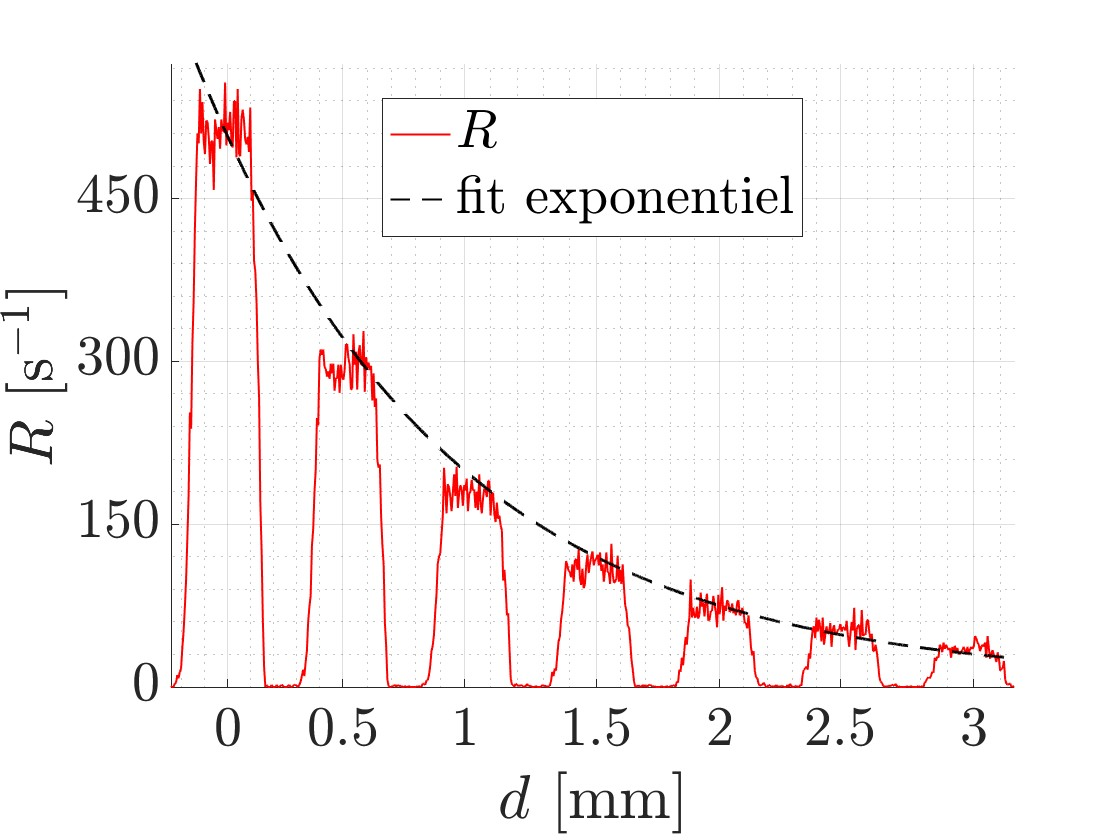
\includegraphics[scale=0.15]{Graphes/nv_epaissuer.jpg}
    \captionsetup{justification=centering}
    \caption{Réponse du tube G-M en fonction de l'épaisseur $d$ des plaquettes d’aluminium}
    \label{figAn1}
\end{figure}

\begin{figure}[H]
\begin{subfigure}{0.45\textwidth}  % Réduire la taille pour s'assurer qu'elles tiennent côte à côte
    \centering  % Centrer cette sous-figure
    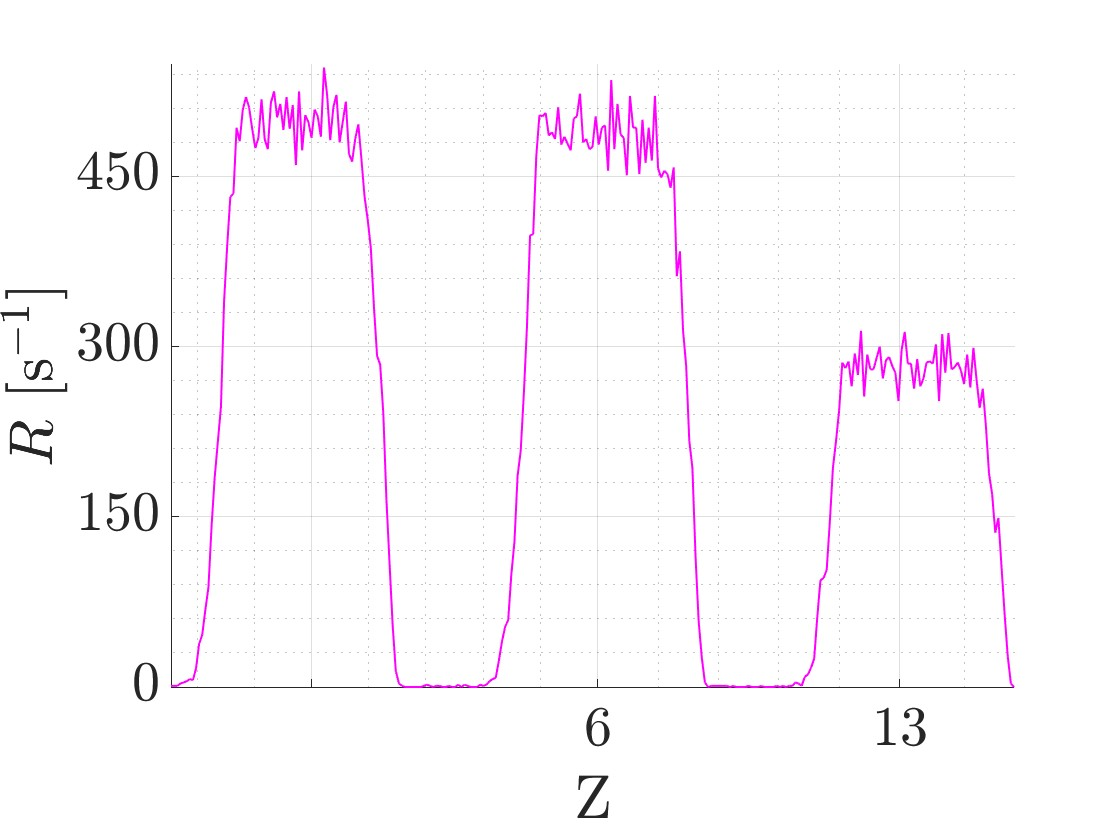
\includegraphics
    [scale=0.15]{Graphes/Annexe_A_Absorption_mat.jpg}
    \captionsetup{justification = raggedright,font = large}
    \caption{}
    \label{figAn2a}
\end{subfigure}
\hspace{0.05\textwidth}
\begin{subfigure}{0.45\textwidth}  % Réduire également ici
    \centering  % Centrer cette sous-figure
    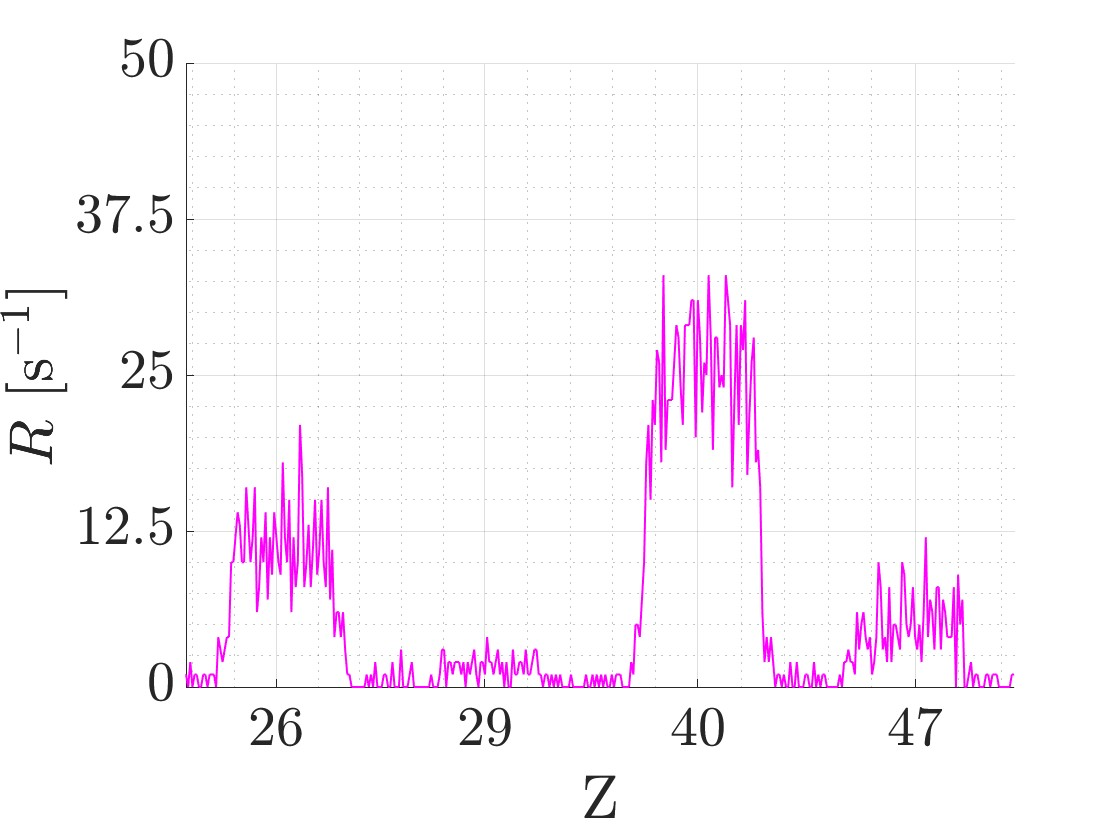
\includegraphics[scale=0.15]{Graphes/Annexe_B_Absorption_mat.jpg}
    \captionsetup{justification = raggedright,font = large}
    \caption{}
    \label{figAn2b}
\end{subfigure}
\vspace{-0.3cm}
\captionsetup{justification=centering}
\caption{Réponse du tube compteur en fonction du numéro atomique des matériaux, qui sont: l’air, $Z=6$, $Z=13$(a) et pour $Z=26$, $Z=29$, $Z=40$, $Z=47(b)$.}
\label{figAn2}
\end{figure}

\end{document}

